\chapter{基于形变梯度的形变子空间构建}
本章将描述构建形变子空间的方法,
并给出了一个基于形变子空间的修改模型形状的算法。
形变子空间构建的输入是一个参考模型和一组形变关键帧。
本文会从每一个形变关键帧中提取出一个特征向量,
作为形变子空间的基向量。
这个特征向量描述的形变关键帧相对于参考模型的相对形变,
由模型中各三角面片的形变梯度组成。
由所有特征向量张成的空间被称为模型的特征空间,
空间中向量均可由基向量非线性插值得到。
特征空间中的向量对应的形变模型组成了模型的形变子空间。
本文还给出了一个基于形变子空间修改模型形状的算法,
可以让用户通过拖动控制点得到符合物体形变特征模型形状。
\section{基于形变梯度的形变子空间}
本文基于网格模型中面片的形变梯度从形变关键帧中提取特征向量,
这些特征向量张成的空间被称作该模型的特征空间。
本节将详细介绍形变梯度的概念,描述特征向量和网格模型互相转换的方法,
以及特征向量在非线性空间进行插值的方法。
\subsection{形变梯度}
形变梯度是一组三维点在三维空间中发生的仿射变换的雅可比矩阵。
参考模型即未发生形变的模型,在本文中即第三章中重建的三维模型。
本文描述的形变梯度是在三角面片上定义的。
Sumner的相关工作\cite{sumner2004deformation}曾经用形变梯度进行模型间的形变转移。
本文中形变子空间构建的方法借鉴了Sumner的MeshIK\cite{sumner2005mesh}。

将三角面片发生的仿射变换记为$\Phi$:
\begin{equation}
    \label{eq_at}
    \Phi(\bm{v})=\bm{T}\bm{v}+\bm{t}
\end{equation}
其中$3 \times 3$矩阵$\bm{T}$包含了旋转变换、缩放变换和斜切变换,
三维向量$\bm{t}$包含了三维空间中的平移变换;
$\bm{v}$为三维空间中的点。
可以看出$\Phi$关于三维向量$\bm{v}$的梯度为变换矩阵$\bm{T}$。
\begin{figure}
    \centering
    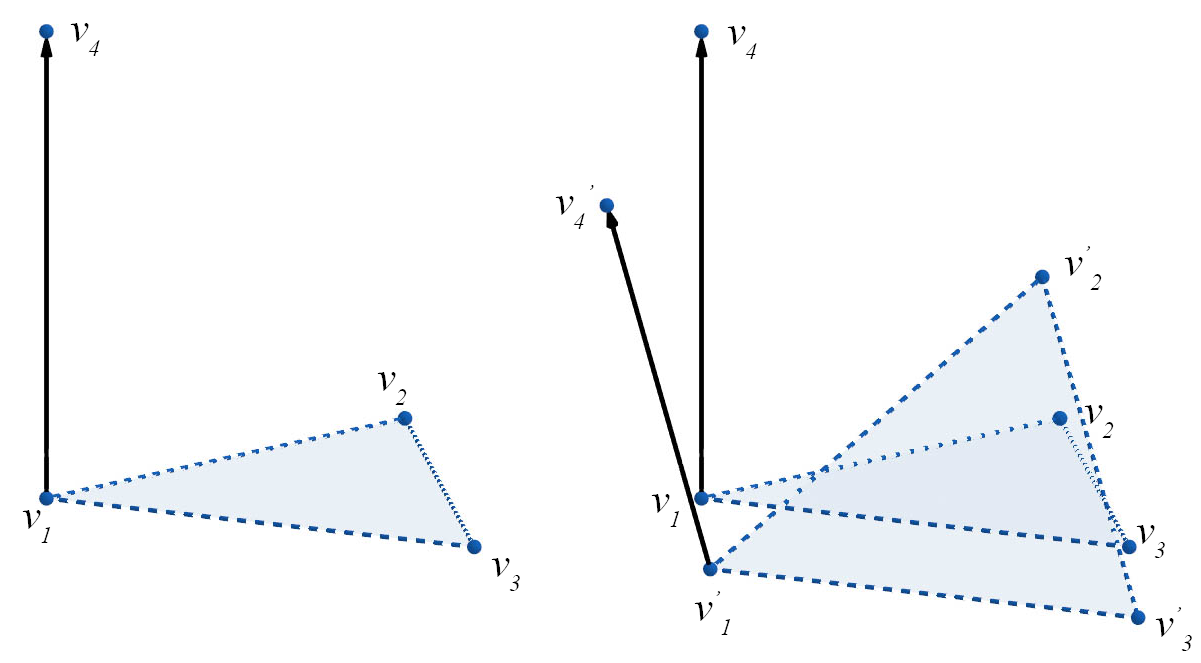
\includegraphics[width = 0.8\textwidth]{./Pictures/DefGra.png}
    \caption{三角面片的顶点四元组}
    \label{deformation_gradient}
\end{figure}

三角面片包含三个不共线的点$\bm{v_1}$、$\bm{v_2}$、$\bm{v_3}$,
但这三个点不足以定义三维空间中的放射变换,
因为这一组点无法定义面片法线方向上的上缩放变换。
所以计算形变梯度时需要加入第四个点$\bm{v_4}$,
组成该面片的顶点四元组。
\begin{equation}
    \bm{v_4}=\bm{v_1}
    +
    \frac
        {(\bm{v_2}-\bm{v_1})\times(\bm{v_3}-\bm{v_1})}
        {\sqrt{|(\bm{v_2}-\bm{v_1})\times(\bm{v_3}-\bm{v_1})|}}
\end{equation}
可以看出$\bm{v_{14}}=\bm{v_4}-\bm{v_1}$是垂直于面片的向量。
$\bm{v_{14}}$的方向通过$\bm{v_{12}}=\bm{v_2}-\bm{v_1}$和
$\bm{v_{13}}=\bm{v_3}-\bm{v_1}$的外积计算得到;
$\bm{v_{14}}$的长度为$\sqrt{|(\bm{v_2}-\bm{v_1})\times(\bm{v_3}-\bm{v_1})|}$,
这保证当面片发生仿射变换时,
$\bm{v_{14}}$会与$\bm{v_{12}}$和$\bm{v_{13}}$等比缩放。
仿射变换后的四个点分别为$\bm{v_1^{'}}$、$\bm{v_2^{'}}$、$\bm{v_3^{'}}$、$\bm{v_4^{'}}$。
若只考虑这四点的相对位置,则平移向量$\bm{t}$为0。
分别将$\bm{v_{41}}$、$\bm{v_{42}}$、$\bm{v_{43}}$代入公式\ref{eq_at},
得到
\begin{equation}
    \begin{aligned}
        &\bm{v_1^{'}}-\bm{v_4^{'}}=\bm{T}(\bm{v_1}-\bm{v_4})\\
        &\bm{v_2^{'}}-\bm{v_4^{'}}=\bm{T}(\bm{v_2}-\bm{v_4})\\
        &\bm{v_3^{'}}-\bm{v_4^{'}}=\bm{T}(\bm{v_3}-\bm{v_4})
    \end{aligned}
\end{equation}
以上方程组可改写成矩阵形式$\bm{V^{'}}=\bm{T}\bm{V}$,
其中
\begin{eqnarray}
     \bm{V}    &=&[\bm{v_1}-\bm{v_4},\bm{v_2}-\bm{v_4},\bm{v_3}-\bm{v_4}] \nonumber \\
     \bm{V^{'}}&=&[\bm{v_1^{'}}-\bm{v_4^{'}},\bm{v_2^{'}}-\bm{v_4^{'}},\bm{v_3^{'}}-\bm{v_4^{'}}]
\end{eqnarray}
$\bm{V}$与$\bm{V^{'}}$均为$3 \times 3$的矩阵,每一列分别为三个相对向量。
由此可以得到三角面片的形变梯度$\bm{T}$
\begin{eqnarray}
    \label{eq_def_grad}
    \bm{T}
    &= &\bm{V^{'}}\bm{V^{-1}} \nonumber \\
    &= &[\bm{v_1^{'}}-\bm{v_4^{'}},\bm{v_2^{'}}-\bm{v_4^{'}},\bm{v_3^{'}}-\bm{v_4^{'}}]\cdot \nonumber \\
    &\ &[\bm{v_1}-\bm{v_4},\bm{v_2}-\bm{v_4},\bm{v_3}-\bm{v_4}]^{-1}
\end{eqnarray}
\subsection{基于形变梯度的特征向量}\label{sec_feature}
本文会从每一个形变关键帧中提取一个基于面片形变梯度的特征向量。
给定一个参考模型$\bm{P}$和一个形变关键帧$\bm{K}$,
它们都包含$n$个顶点和$m$个面片。
对于$\bm{K}$中的每一个面片,都可以计算出相应的形变梯度$\bm{T}$。
由公式\ref{eq_def_grad}可知,当参考模型中的顶点位置确定,即为常数时,
形变梯度$\bm{T}$中各元素的值均为形变模型(形变关键帧)中相应顶点坐标元素的线性组合。
所以可用如下矩阵乘法计算模型的特征向量:
\begin{equation}
    \label{eq_mat_get_f}
    \bm{f}=\bm{G}\bm{x}
\end{equation}
其中向量$\bm{x}=(x_1,...,x_{n+m},y_1,...,y_{n+m},z_1,...,z_{n+m}) \in \mathbb{R}^{3(n+m)}$
是是$n+m$个三维点的坐标值堆叠成长向量,
其中$n$个点为模型中的顶点,$m$个点为$m$个面片的第四点。
线性算子$\bm{G}$的元素的值仅由参考模型中顶点的位置决定,
它用于构造特征向量$\bm{f}\in\mathbb{R}^{9m}$。
特征向量$\bm{f}$由$m$个面片的形变梯度$\bm{T}$中的元素的值堆叠而成。
矩阵乘法$\bm{Gx}$根据公式\ref{eq_def_grad}计算了每个面片的形变梯度$\bm{T}$,
并将这$m$个$3 \times 3$矩阵中的元素堆叠到长向量$\bm{x}$中的元素的值堆叠而成。

线性算子$\bm{G}$为$9m\times 3(n+m)$的矩阵。
由公式\ref{eq_def_grad}可知,
每个顶点只会影响包含它的面片的形变梯度,
所以矩阵$\bm{G}$是一个稀疏矩阵。
且每一个顶点在不同维度的值在运算中具有相同的线性组合,
所以矩阵$\bm{G}$拥有如下对角分块的结构
\begin{equation}
    \bm{G}=
    \begin{bmatrix}
        \bm{G_d} &        & \\ 
         &       \bm{G_d} & \\ 
         &       &        \bm{G_d}
    \end{bmatrix}
\end{equation}
每个矩阵块$\bm{G_d}$是一个$3m \times (n+m)$的稀疏矩阵,
每一行仅有四个非零元素,
分别对应利用公式\ref{eq_def_grad}计算相应形变梯度时需要的四个顶点。
求解公式\ref{eq_mat_get_f}中的方程就可以从特征向量映射回顶点坐标。
但是由于特征向量与模型在空间中平移无关,
所以直接求解公式\ref{eq_mat_get_f}$\bm{x}$会有无穷多个解。
要求解$\bm{x}$需要确定或约束至少一个顶点的位置。
约束顶点的方法将在网格修改模型的章节中介绍。
\subsection{特征向量的非线性插值}
本文将从每个形变关键帧中提取出特征向量称为基向量,
将基向量张成的向量空间称为模型的特征空间,
特征空间中的向量对应的形变模型是本文认为合理的形变模型。
特征空间中的向量均可由基向量插值得到。
对于$k$个基向量,给定$k$维权重向量$\bm{w}$,
可得到插值后的特征向量
\begin{equation}
    \bm{f_w}=\bm{Intp}(\bm{w})
\end{equation}
其中$\bm{Intp}$为插值函数。

线性插值是最为常见的向量插值方法,
但并不适用于本文中特征向量的插值。
由于本文中特征向量是表示模型姿态的变换矩阵$\bm{T}$的线性变换,
所以对特征向量线性插值等价于对模型的姿态线性插值。
当变换矩阵$\bm{T}$中包含旋转时,
插值后的模型姿态会显得不自然。
这种姿态在旋转程度较大时尤为明显,
如图\ref{linear_vs_unlinear}(三)所示。
在本文的应用场景中,
只有当选取形变关键帧密集采样,
使得相近的关键帧中面片间仅有微小的旋转时,
线性插值才适用于特征向量的插值。
但这样的密集采样并不现实,
也使得形变子空间的构建失去了意义。
为了解决插值结果不自然的问题,
本文需要一种能够将旋转分量更自然的插值的方法将基向量张成特征空间。
本文采用的是一种基于极分解(polar decomposition)\cite{shoemake1992matrix}
和矩阵指数映射( matrix exponential map)\cite{murray2017mathematical}
\cite{trove.nla.gov.au/work/222715717}
的非线性插值方法。
图\ref{linear_vs_unlinear}中前两张图为两个形变关键帧,
用$1:1$的权重对二者的特征向量插值,
后两张图分别为线性插值和非线性插值的结果。
模型的特征空间就是由基向量通过这种插值方法张成的。
\begin{figure}
    \centering
    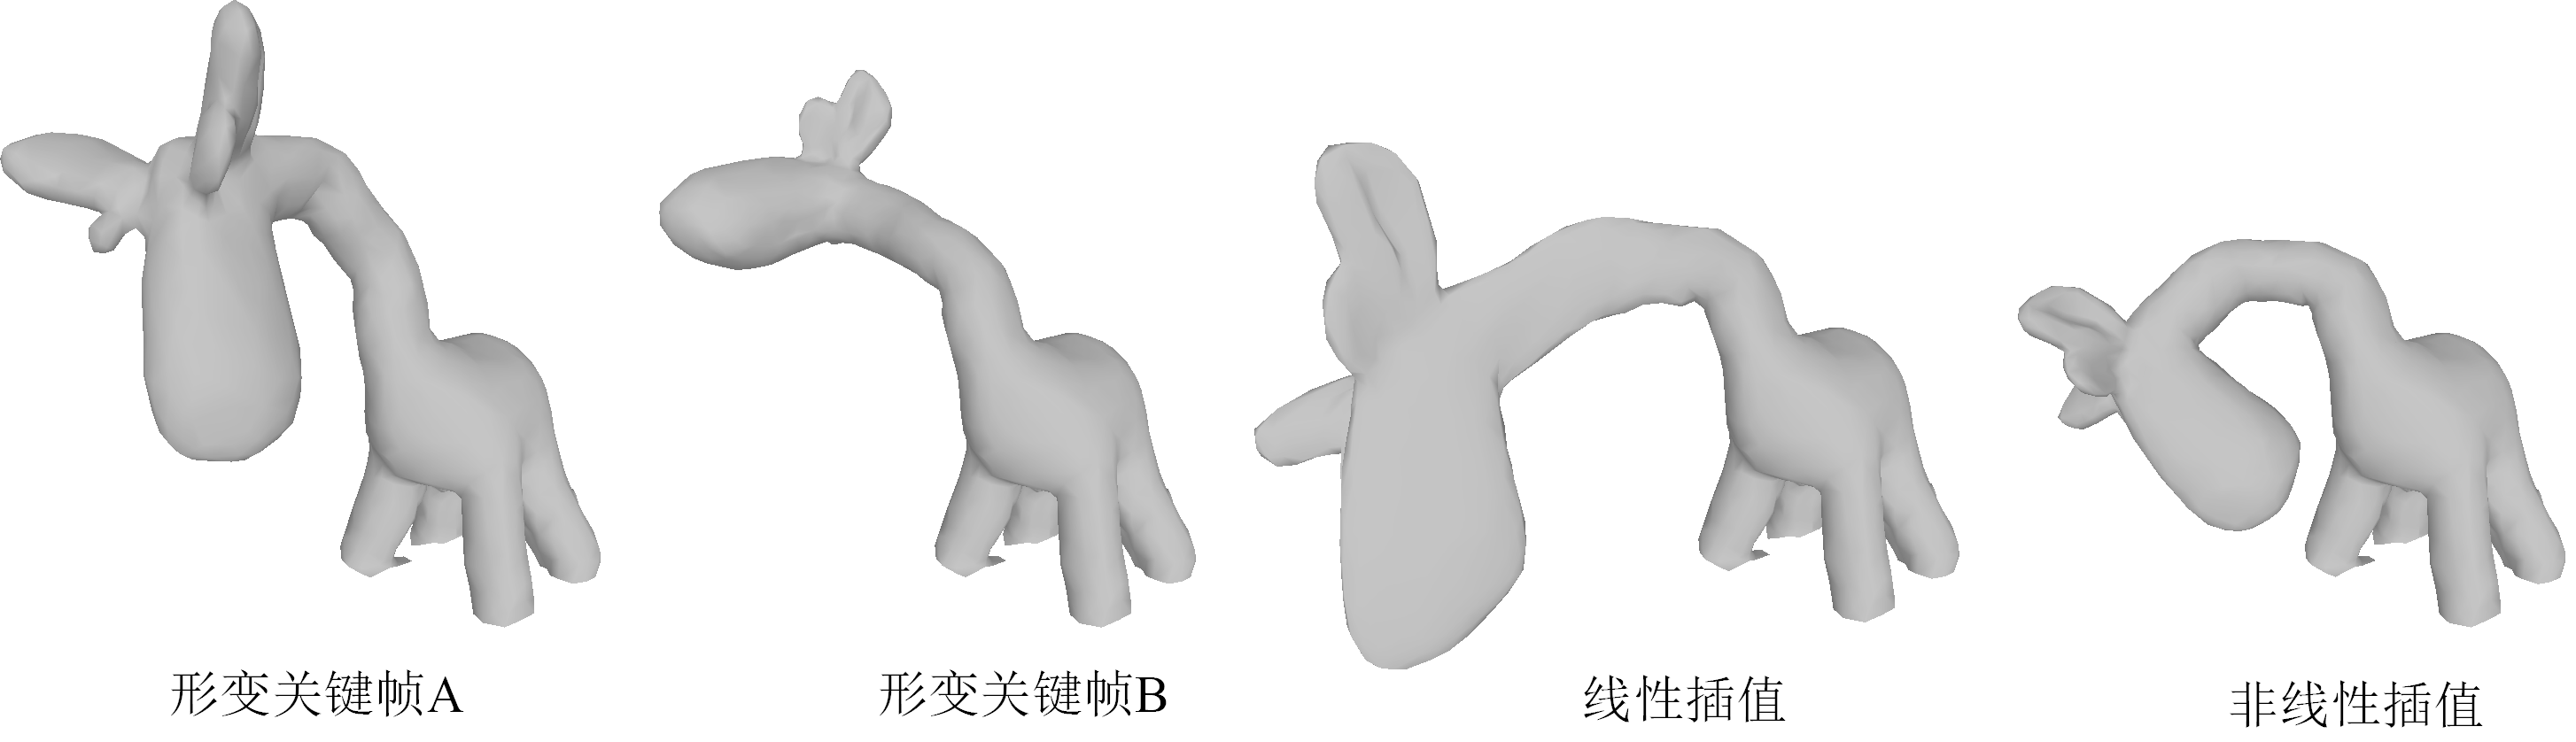
\includegraphics[width = \textwidth]{./Pictures/linear_vs_unlinear.png}
    \caption{特征的向量的插值方法}
    \label{linear_vs_unlinear}
\end{figure}

首先,用极分解将第$i$个形变关键帧中的第$j$个面片的形变梯度$\bm{T_{ij}}$
分解为旋转和缩放/切边两个部分:
\begin{equation}
    \bm{T_{ij}}=\bm{R_{ij}S_{ij}}
\end{equation}
这两部分会采用不同的插值策略。
其中缩放/切变部分$\bm{S_{ij}}$可直接使用线性插值,
而旋转部分$\bm{R_{ij}}$则需要做特殊处理。

本文在旋转分量的插值中运用了矩阵的指数映射和对数映射。
本节将简要介绍矩阵指数映射和对数映射的概念,
想了解更多细节和证明可查阅相关资料\cite{murray2017mathematical}
\cite{trove.nla.gov.au/work/222715717}。
这两种映射能够提供空间旋转在$\bm{SO}(3)$和$\mathfrak{so}(3)$间的转换。
其中$\bm{SO}(3)$为一个李群,称为三维旋转群,
是特殊正交群$\bm{SO}(n)$在$n=3$时的特例,
它包含了所有三维旋转矩阵。
$\mathfrak{so}(3)$为三维旋转群$\bm{SO}(3)$对应的李代数。
可以看做一组$3 \times 3$的反对称矩阵,
这些矩阵可有一个向量生成,
这个向量是三维正交群中的旋转矩阵对应旋转向量,
它们的对应关系可由罗德里格斯公式表明。
所以$\mathfrak{so}(3)$也可以看做是三维旋转向量组成的空间。
指数映射可以将$\bm{SO}(3)$中的旋转矩阵映射到$\mathfrak{so}(3)$,
对数映射为指数映射的逆映射。
在本文采用的插值方法中,
会利用指数映射将旋转矩阵从$\bm{SO}(3)$映射到$\mathfrak{so}(3)$,
在$\mathfrak{so}(3)$中做线性插值,然后将插值的结果用对数映射映射回
$\bm{SO}(3)$。
模型中第$j$个面片的形变梯度$\bm{T_j}$的非线性插值可由如下公式描述:
\begin{equation}
    \label{eq_unlinear}
    \bm{T_j}(\bm{w})
    =
        exp(\sum_{i=1}^{k}w_i\log (\bm{R_{ij}}))
        \cdot
        \sum_{i=1}^{k}w_i\bm{S_{ij}}
\end{equation}
其中$exp$和$log$分别为指数映射和对数映射,$w_i$为第$i$个基向量的权重。
特征向量中各面片的形变梯度均使用公式\ref{eq_unlinear}进行非线性插值,
即为特征向量的插值函数$\bm{Intp}(\bm{w})$。
\section{基于形变子空间的网格模型形状修改}
本节交描述一个基于形变子空间的模型修改方法。
用户可通过拖动控制点实现对模型形状的修改。
\subsection{形状优化模型}
如章节\ref{sec_feature}所述,
由于特征向量与模型的平移无关,
所以需要多模型中至少一个顶点的位置进行约束,
才能得到与指定特征向量对应的形变模型。
这可以用如下优化问题表示:
\begin{eqnarray}
    \bm{x}&=&arg\ \min_{\bm{x}} (E_f(\bm{x}) + E_c(\bm{x})) \nonumber \\
          &=&arg\ \min_{\bm{x}} (\|\bm{Gx}-\bm{f}\| + \lambda_c  \sum_{i=1}^{l}\|\bm{v_i}-\bm{vc_i}\|)
\end{eqnarray}
其中$E_f$为特征约束,可由公式\ref{eq_def_grad}得到,
将模型约束在形变空间内;
$E_c$为控制点约束,$\bm{vc_i}$为固定点的位置。
优化结果即为指定了固定点后特征向量$\bm{f}$对应的形变模型的顶点位置。
$E_c(\bm{x})$可改写为与$E_f$类似的矩阵形式:
\begin{eqnarray}
    E_c(\bm{x})&=&\|\bm{
        \bm{M_c}x}
        -
        \bm{f_c}\| \nonumber \\
    \bm{M_c}&=&
    \begin{bmatrix}
        \bm{G_c} &        & \\ 
         &       \bm{G_c} & \\ 
         &       &        \bm{G_c}
    \end{bmatrix}
\end{eqnarray}

当有$l$个固定点时,$\bm{G_c}$为$l \times (n+m)$的矩阵,
每行只有与固定点$\bm{v_i}$对应的一列非零,
值为权重$\lambda$。
$\bm{f_c}$为$3l$维的向量,
对应$3l$个固定点的坐标,
值为对应固定点坐标与固定点权重$\lambda$的乘积。
因为$E_f$与$E_c$有如此相近的形式,
可以将二者合并为一个能量。
有此可以得到新的优化问题:
\begin{equation}
    \label{eq_feature2mesh}
    \bm{x}=arg\ \min_{\bm{x}} \| \bm{\widetilde{G}x}-(\widetilde{\bm{f}}+\bm{c}) \|
\end{equation}
其中$\bm{\widetilde{G}}$为扩展后的$\bm{G}$,$\widetilde{f}$为扩展后的$\bm{f}$。
\begin{eqnarray}
    \bm{\widetilde{G}}&=&
    \begin{bmatrix}
        \bm{\widetilde{G_d}} &        & \\ 
         &       \bm{\widetilde{G_d}} & \\ 
         &       &                  \bm{\widetilde{G_d}}
    \end{bmatrix}\\
    \bm{\widetilde{G_d}}&=&
    \begin{bmatrix}
        \bm{G_d} \\ 
        \bm{G_c}
    \end{bmatrix}
\end{eqnarray}

若将公式\ref{eq_feature2mesh}中的$\bm{f}$替换为$\bm{f_w}=\bm{Intp}(\bm{w})$,
并将插值权重$\bm{w}$也作为优化变量,
以用户指定的控制点作为静止点,
就能得到修改模型形状的优化问题:
\begin{equation}
    \bm{x}=arg\ \min_{\bm{x},\bm{w}}
    \|
        \bm{\widetilde{G}x}
        -
        (\bm{Intp}(\widetilde{\bm{f}})+\bm{c}) 
    \|
\end{equation}
\section{本章小结}